\begin{frame}
\begin{center}
\emph{Project 1}\\\vspace{1em}
\emph{\Large{Measuring Moralization in Political Attitude Expression}}\\\vspace{1em}
\emph{Conditionally accepted at the \textit{Journal of Politics}}
\end{center}
\end{frame}


\begin{frame}
\frametitle{Open-ended survey response in 2012 ANES}
\begin{exampleblock}{Is there anything in particular about [Candidate] that might make you want to vote for him? What is that?}
  \begin{center}
    \textit{``I think he represents a far more healthy vizsion for the country on a lot of levels, economically, environmentally, the vision he represents for the future of the country is much more in line with the country I hope to leave for my grandchildren, socially - protecting the rights of individuals, specifically the rights of women and individuals, the right to choose, picking a Supreme Court Justice and developing a tax system that is fair to everyone. [...]''}
  \end{center}
\end{exampleblock}
\end{frame}


\begin{frame}%[allowframbreaks]
  \frametitle{Questions}
  \begin{itemize}
    \item Do individuals rely on \emph{moral foundations} when evaluating political \emph{parties} and \emph{candidates} \citep{haidt2008moral}?
    \item Are there systematic differences between \emph{liberals} and \emph{conservatives} \citep{haidt2007morality,graham2009liberals}?
    \item Are moral values \emph{determinants} of political thinking, or only a \emph{rhetorical device} that citizens \emph{learn} to bolster their political views?
  \end{itemize}
\end{frame}


\begin{frame}%[allowframbreaks]
  \frametitle{Hypotheses}
  \begin{enumerate}
    \item \emph{Liberals} are more likely to emphasize moral foundations of \emph{harm/care} and \emph{fairness/reciprocity} than conservatives when evaluating political parties and candidates. On the other hand, \emph{conservatives} are more likely to emphasize moral foundations of \emph{ingroup/loyalty}, \emph{authority/respect}, and \emph{purity/sanctity} than liberals.
    \item Individuals who have more experience and are more engaged in the political system (i.e. with higher \emph{political sophistication}, high \emph{media exposure}, frequent \emph{political discussions}, prior \emph{participation}) are more likely to emphasize moral foundations when evaluating political parties and candidates.
  \end{enumerate}
\end{frame}

\subsection{Empirical Analyses}

\begin{frame}%[allowframbreaks]
  \frametitle{Overview}
  \begin{itemize}
    \item 2012 + 2008 American National Election Study (pre-election)
    \item Major dependent variable: \emph{open-ended questions} where respondents were asked what they \emph{liked} and \emph{disliked} about the parties and candidates
    \item Moral Foundations \emph{dictionary} proposed by \citep{graham2009liberals} to look for \emph{signal} words.
    \item Model individual response patterns for each of the moral foundations
  \end{itemize}
\end{frame}


\begin{frame}%[allowframbreaks]
  \frametitle{Analyzing Open-Ended Survey Responses}
\begin{exampleblock}{Is there anything in particular about [Candidate] that might make you want to vote for him? What is that?}
  \begin{center}
    \textit{``I think he represents a far more healthy \underline{vision} for the country on a lot of levels, economically, environmentally, the vision he represents for the future of the country is much more in line with the country I hope to leave for my grandchildren, socially - {\color{blue}protecting} the {\color{green}rights} of {\color{red}individuals}, specifically the {\color{green}rights} of women and {\color{red}individuals}, the right to choose, picking a Supreme Court {\color{green}Justice} and developing a tax system that is {\color{green}fair} to everyone. [...]''}
  \end{center}
\end{exampleblock}
  \begin{itemize}
  \item Moral Foundations: {\color{blue}Harm}, {\color{green}Fairness}, {\color{red}Ingroup}
  \end{itemize}
\end{frame}


\begin{frame}%[allowframbreaks]
  \frametitle{Descriptive Results}
  \begin{figure}[ht]\centering
    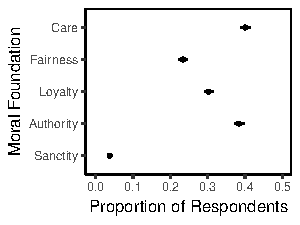
\includegraphics[height=.8\textheight]{fig/prop_mft}
  \end{figure}
\end{frame}


\begin{frame}%[allowframbreaks]
  \frametitle{Predicting References to Moral Foundations}
  \begin{figure}[ht]\centering
    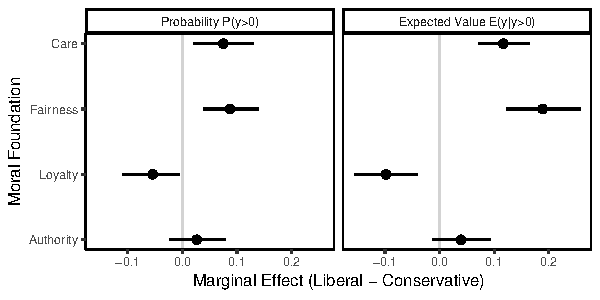
\includegraphics[width=\textwidth]{fig/tobit_ideol}
  \end{figure}
\end{frame}


\begin{frame}%[allowframbreaks]
  \frametitle{Moral Reasoning as a Political Learning Process}
  \begin{figure}[ht]\centering
    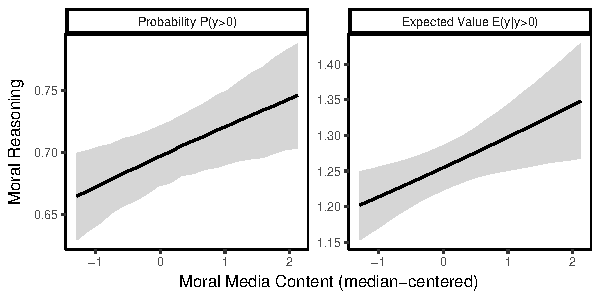
\includegraphics[width=\textwidth]{fig/tobit_media}
  \end{figure}
\end{frame}

\subsection{Discussion}

\begin{frame}%[allowframbreaks]
  \frametitle{Discussion}
  \begin{itemize}
\item Open-ended survey responses provide a useful \emph{unobtrusive measure} to investigate the relationship between moral considerations and political reasoning
\item \emph{Liberals} and \emph{conservatives} differ in their emphasis on moral dimensions
\item Differences not always consistent with \emph{Moral Foundations Theory} (fuzzy measurement etc.)
\item Political \emph{learning} process
\item \emph{Further developments}:
    \begin{itemize}
     \item Revise dictionary
     \item Differentiate between rejection/approval of moral foundations, in-party/out-party, candidate vs. party, etc.
     \item Development over longer time period, effect of polarization
     \item Structural topic models \citep{roberts2014structural}
     \item Experimental designs
    \end{itemize}
  \end{itemize}
\end{frame}


\begin{frame}%[allowframbreaks]
\frametitle{Open-ended survey response in 2012 ANES}
\begin{exampleblock}{Is there anything in particular about [Party] that might make you want to vote against him? What is that?}
  \begin{center}
    \textit{``The party is run by Satan - it's filled with liars, cheaters, murderers, the sexually immoral, etc. Should you reject God in life, I am sure you'll be joined alongside in hell by most [members of party], with all of you fighting to be lord of that domain also.''}
  \end{center}
\end{exampleblock}
\end{frame}
